\thispagestyle{fancy}
	
	\vspace{-2em} % Adjust vertical space as needed
	\begin{center}



\addcontentsline{toc}{subsection}{Message of the Dean, Faculty of Engineering Technology}    
\subsection*{\textsc{Message of the Dean, Faculty of Engineering Technology}}
	\end{center}

   
    
    \begin{wrapfigure}{l}{0.3\textwidth}
		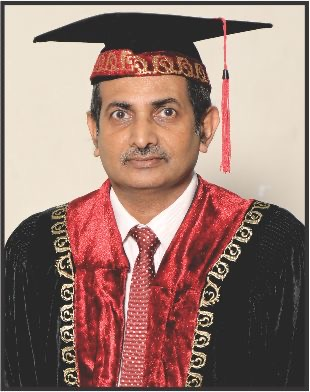
\includegraphics[width=0.3\textwidth]{Images/DeanFET.jpeg}
	\end{wrapfigure}
	\vspace{2em} % Adjust vertical space as needed




		It is a great pleasure to have an opportunity to convey my best wishes to the 8th International Research Symposium (IRS-2024) of the University of Vocational Technology. I want to express how proud I am of the hard work you have all put into your research works. This event highlights the diversity of ideas and perspectives that enrich our community, allowing us to learn from one another and discover new approaches to the important challenges we face today.
        
This symposium is not just about presenting your work; it is also a fantastic opportunity to share ideas and engage in meaningful conversations. Connecting with fellow researchers and industry professionals can spark innovative ideas and lead to valuable collaborations. Remember, the insights you gain from each other can inspire new directions in your research and open doors to exciting possibilities.

As you present your research, keep in mind that the journey of discovery is just as important as the results. Embrace the spirit of exploration and creativity that drives your work. Consider how your findings can contribute to broader conversations in your field and make a positive impact in the community. I am excited to hear about the remarkable work you have accomplished and to see the engaging discussions that will take place throughout the symposium. Together, we can celebrate our achievements and inspire one another to reach even greater heights.

	\vspace{1cm}
	\noindent
	Dr. Jayalal Wettasinghe\\
Dean\\
Faculty of Engineering Technology
	
	\newpage